\section{Recipes}

The \gls{api}-level rules that are enforced by Sensei are called recipes.
This name is chosen to emphasize the difference between Sensei and existing, traditional security tools, who often use rules to scan for vulnerabilities.
Recipes are also commonly used in the \gls{devops} movement, for example by the popular automation tool Chef~\footnote{\url{https://www.chef.io/}}.

\subsection{Creating recipes}
Customization and distribution of the recipes is a crucial feature for any successful tool supporting the paved path methodology.
If the recipes are easy to customize, it ensures that Sensei can provide highly relevant and applicable feedback to the developer.
This customization should be scalable and hence not be a service provided by us.
It should allow developers and security experts to effortlessly share project-specific or team-specific guidelines among each other.
For this reason, the recipe creation process should be easy and fast, and at the same time versatile. 

Our first approach allowed users to create new recipes through predefined recipe models.
A \gls{gui} was used to let the recipe writer fill in a number of variables for this model.
A simple example of such a model is  the ``Replace method call model”.
Figure~\ref{fig:recipeedit2} shows a recipe being created to replace the \texttt{addCookie} method with a safe alternative from the \gls{owasp} \gls{esapi}, an open-source, web application security control library designed to make secure development easier~\cite{ESAPI}; the organization also provides some commonly used security guidelines.
The recipe writer has to fill in some specifics about the method they want to be marked by Sensei, such as the package, class, and method names.
Then they can write one or more quick-fixes.
Here, they have to create a quick-fix description and they have to define the code fragment that will be used to replace the original.
To do so they can reuse arguments, method names, and more from the original code by means of a template language.
In the field ``Rewrite to", the example quick-fix reuses the first argument of the original method call by using the template \texttt{arguments.0}. 

\begin{figure}
  \centering
  %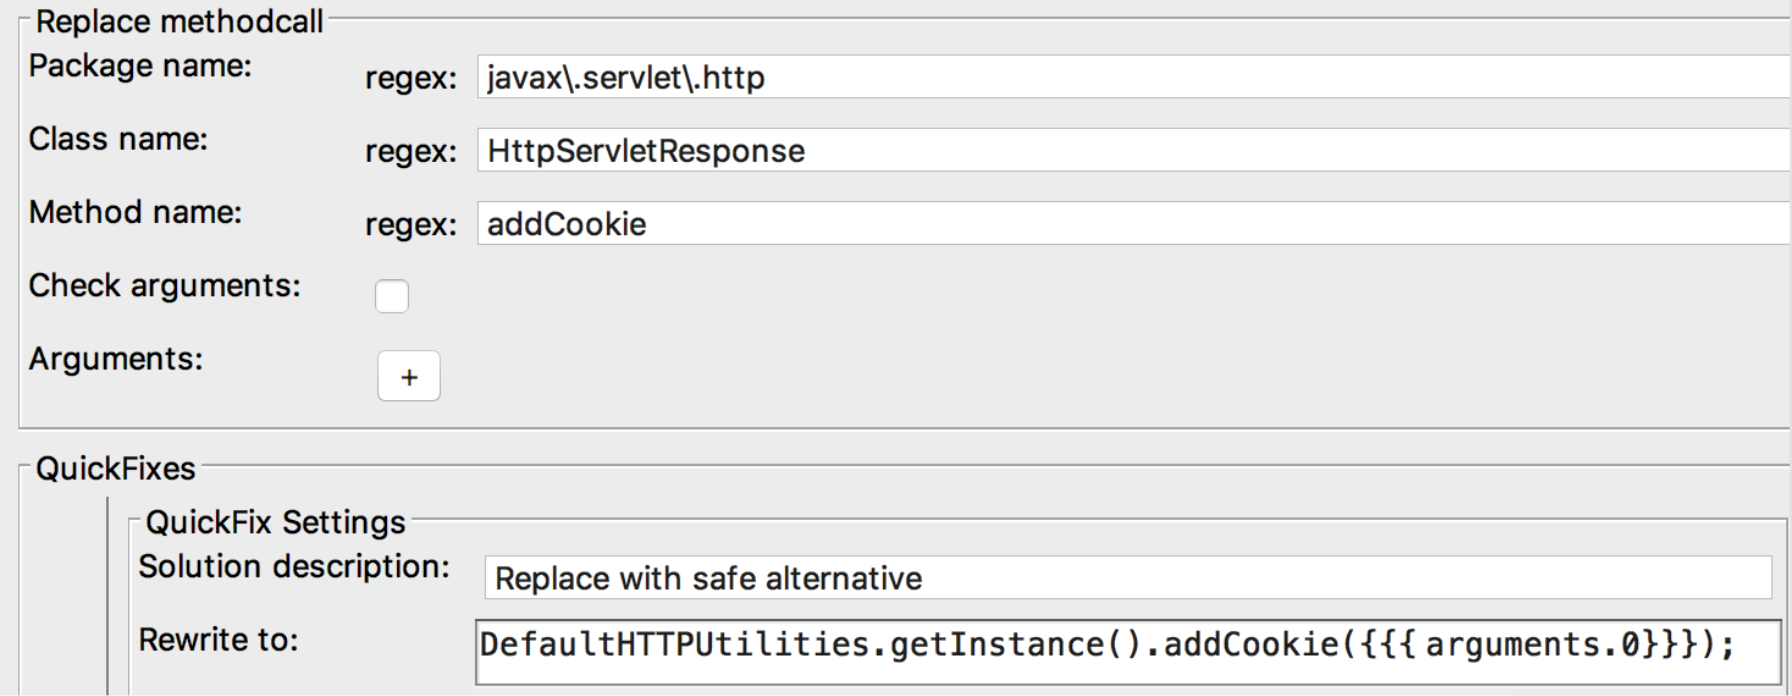
\includegraphics[width=\textwidth]{ruleedit2.png}
  \includegraphics[width=\textwidth,page=7]{04-tools/figures/figures2.pdf}
  \caption[Old model-based recipe editor]{The old recipe editor used a \gls{gui}. It required the recipe writer to fill in a number of input fields to specify the behaviour of the recipe.}
  \label{fig:recipeedit2} 
\end{figure}

However, for more complex models the number of input fields grew rapidly to accommodate a plethora of corner cases, and so did the number of models for multiple scenarios.
As of now the old recipe editor has over 40 different models.
With this many models, it becomes overwhelming for recipe writers that have to select a model to enforce their desired coding guideline.
The described model-based recipe creation process is not flexible and intuitive enough, so in the next iteration a new approach was taken.

In the new approach we split up the recipe in two parts: A trigger to identify the violation, plus an optional quick-fix to correct the vulnerability consistently according to company best practices.
Triggers are now specified by way of \gls{yaml}\footnote{\url{https://yaml.org/}} syntax, which provides more flexibility.
To develop this \gls{yaml} syntax, all existing Sensei rules were analyzed and grouped based on which elements in the code are incorrect and which transformations are required to fix them.
The resulting taxonomy of 10 bad code patterns is included in Appendix~\ref{app:patterns}.

Since this approach requires recipe writers to learn the new syntax, we have provided some tools to assist them, in the form of a \gls{gui} that can be used to build the desired recipe from scratch.
In addition, the recipe editor is now more context-aware.
The recipe writer can open a recipe creation wizard by pressing a key combination in the text editor in the \gls{ide} and selecting ``create new recipe".
This opens a context-aware menu depending on the position of the caret.
For example, if the caret was on a method call, the menu contains an option to create a new recipe that searches for similar method calls, as shown in Figure~\ref{fig:newrecipemethodcall}.

\begin{figure}[t]
  \centering
  %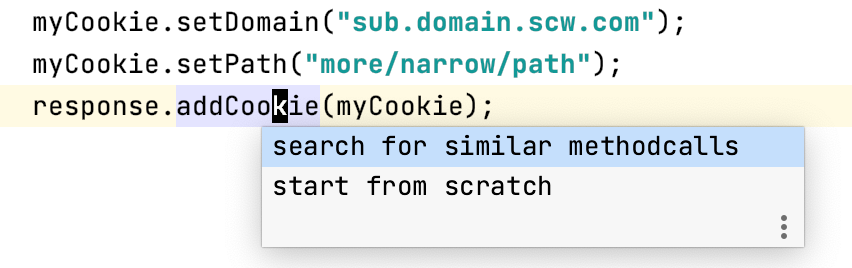
\includegraphics[width=0.8\textwidth]{rulewizard2.png}
  \includegraphics[width=0.8\textwidth,page=11]{04-tools/figures/figures2.pdf}
  \caption[Context-aware recipe creation menu]{The recipe creation menu is context aware, its options will change based on the caret position.}
  \label{fig:newrecipemethodcall} 
\end{figure}

When this context-aware option is chosen, the recipe creation wizard is opened and a recipe is automatically suggested from the available context.
To search for a methodcall, the information that can be pre-filled from context is the type and the name of the methodcall, as well as the number of arguments and each of their types.
The user can then adjust the recipe to reach the desired results through the \gls{yaml} code or the provided \gls{gui}.
This window also provides a preview panel, as shown in Figure~\ref{fig:recipewizard1}.
In this panel, the code file from which the recipe wizard was opened is shown, and the effects of the recipe being created are visualised, which allows for easy customization.

\begin{sidewaysfigure}
  \centering
  %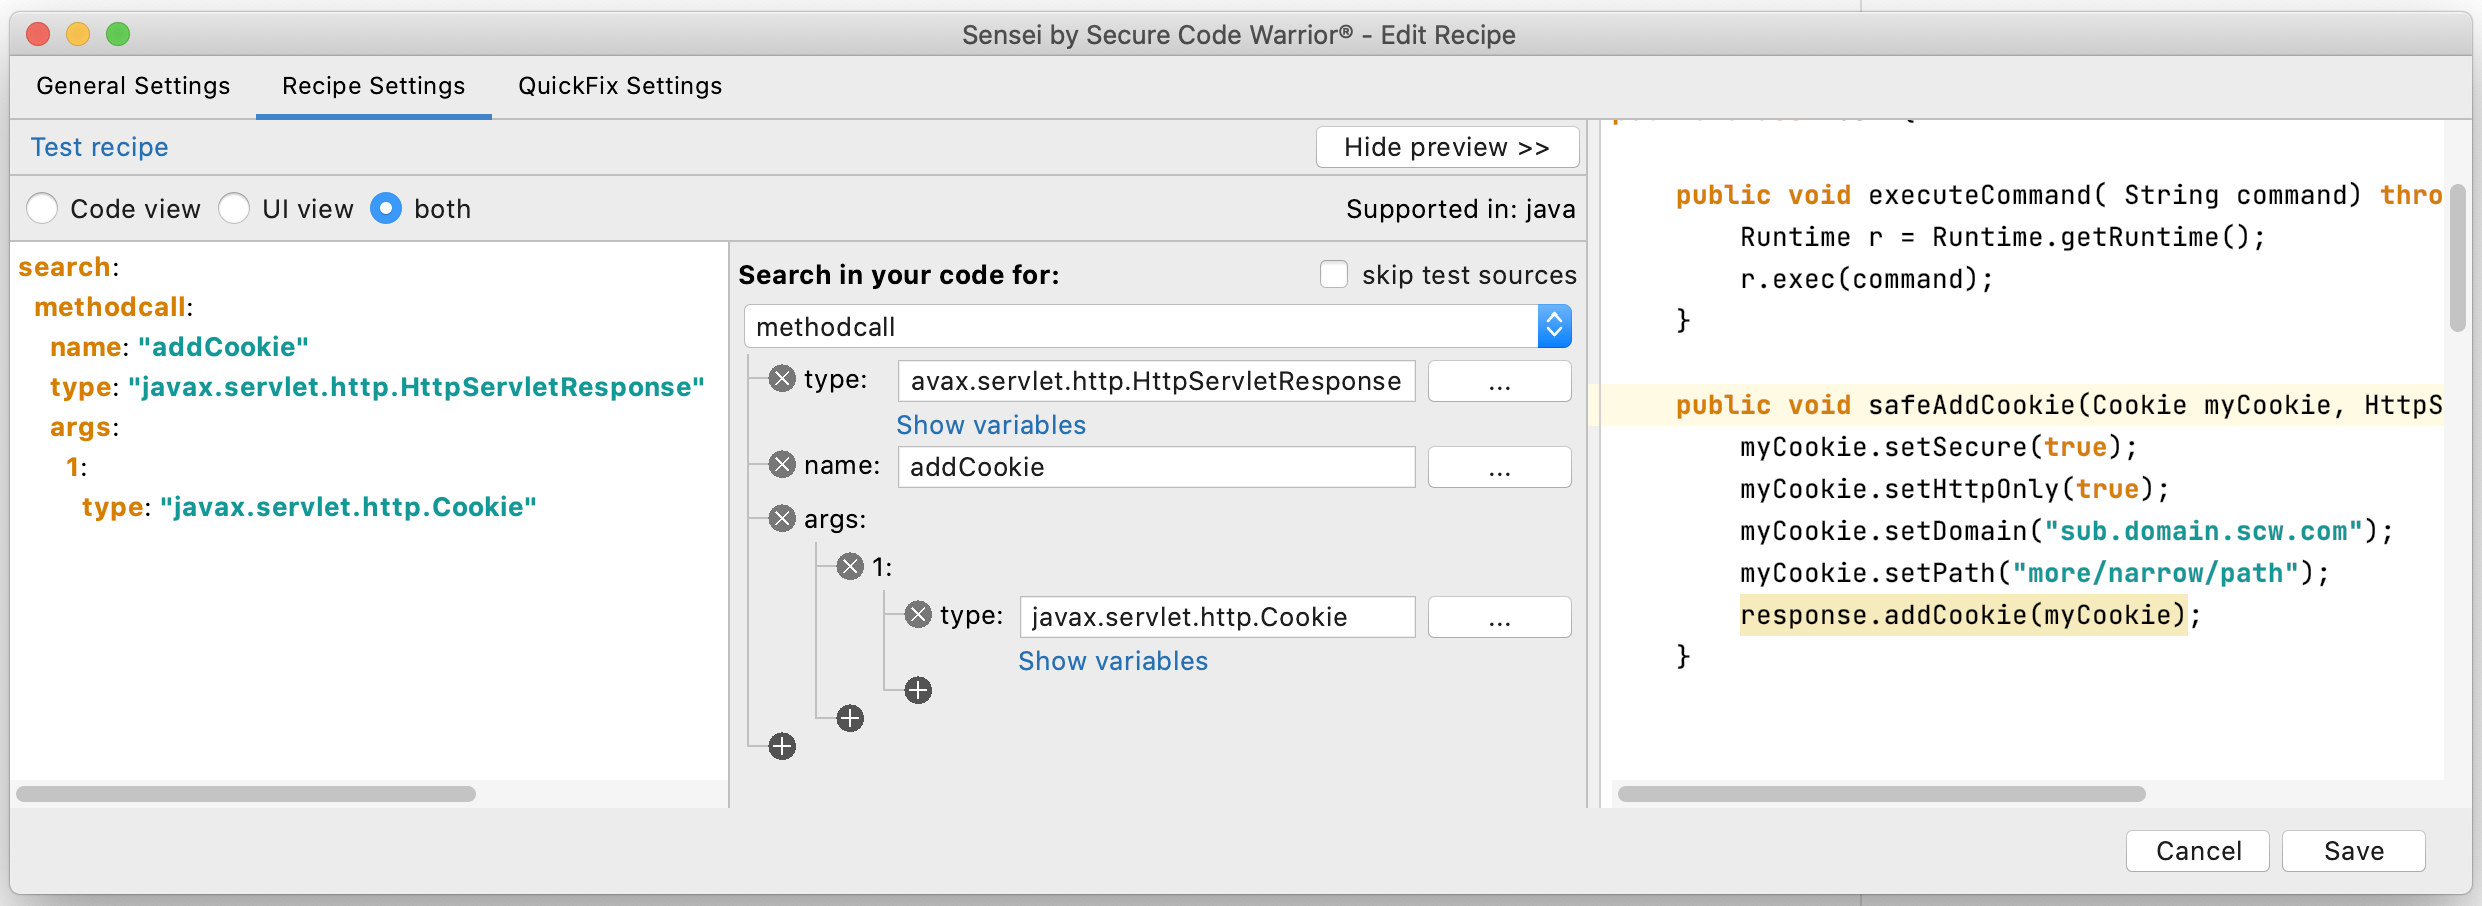
\includegraphics[width=\textwidth]{rulewizard1.png}
  \includegraphics[width=\textwidth,page=10]{04-tools/figures/figures2.pdf}
  \caption[Recipe created from context]{A recipe created through the ``search for similar methodcalls" option in the context-aware recipe creation menu will generate a \gls{yaml}-based recipe with details from the context of the caret position.}
  \label{fig:recipewizard1} 
\end{sidewaysfigure}

After creating a trigger, it is possible to create an optional quick-fix.
Here, the recipe writer has to fill in the quick-fix description and the replacement code.
For the replacement code, they can make use of the same template language as in the first approach to reuse parts of the original code.
Below the input field, an overview is provided of the available parts of the original code, as shown in Figure~\ref{fig:createfix}.
Double clicking one of these options, adds its template to the fix.
The quick-fix creation window also offers a live preview in the lower right corner that highlights the changes that would be made to the original code (shown in the lower left corner) if the quick-fix is applied.

\begin{figure}
  \centering
  %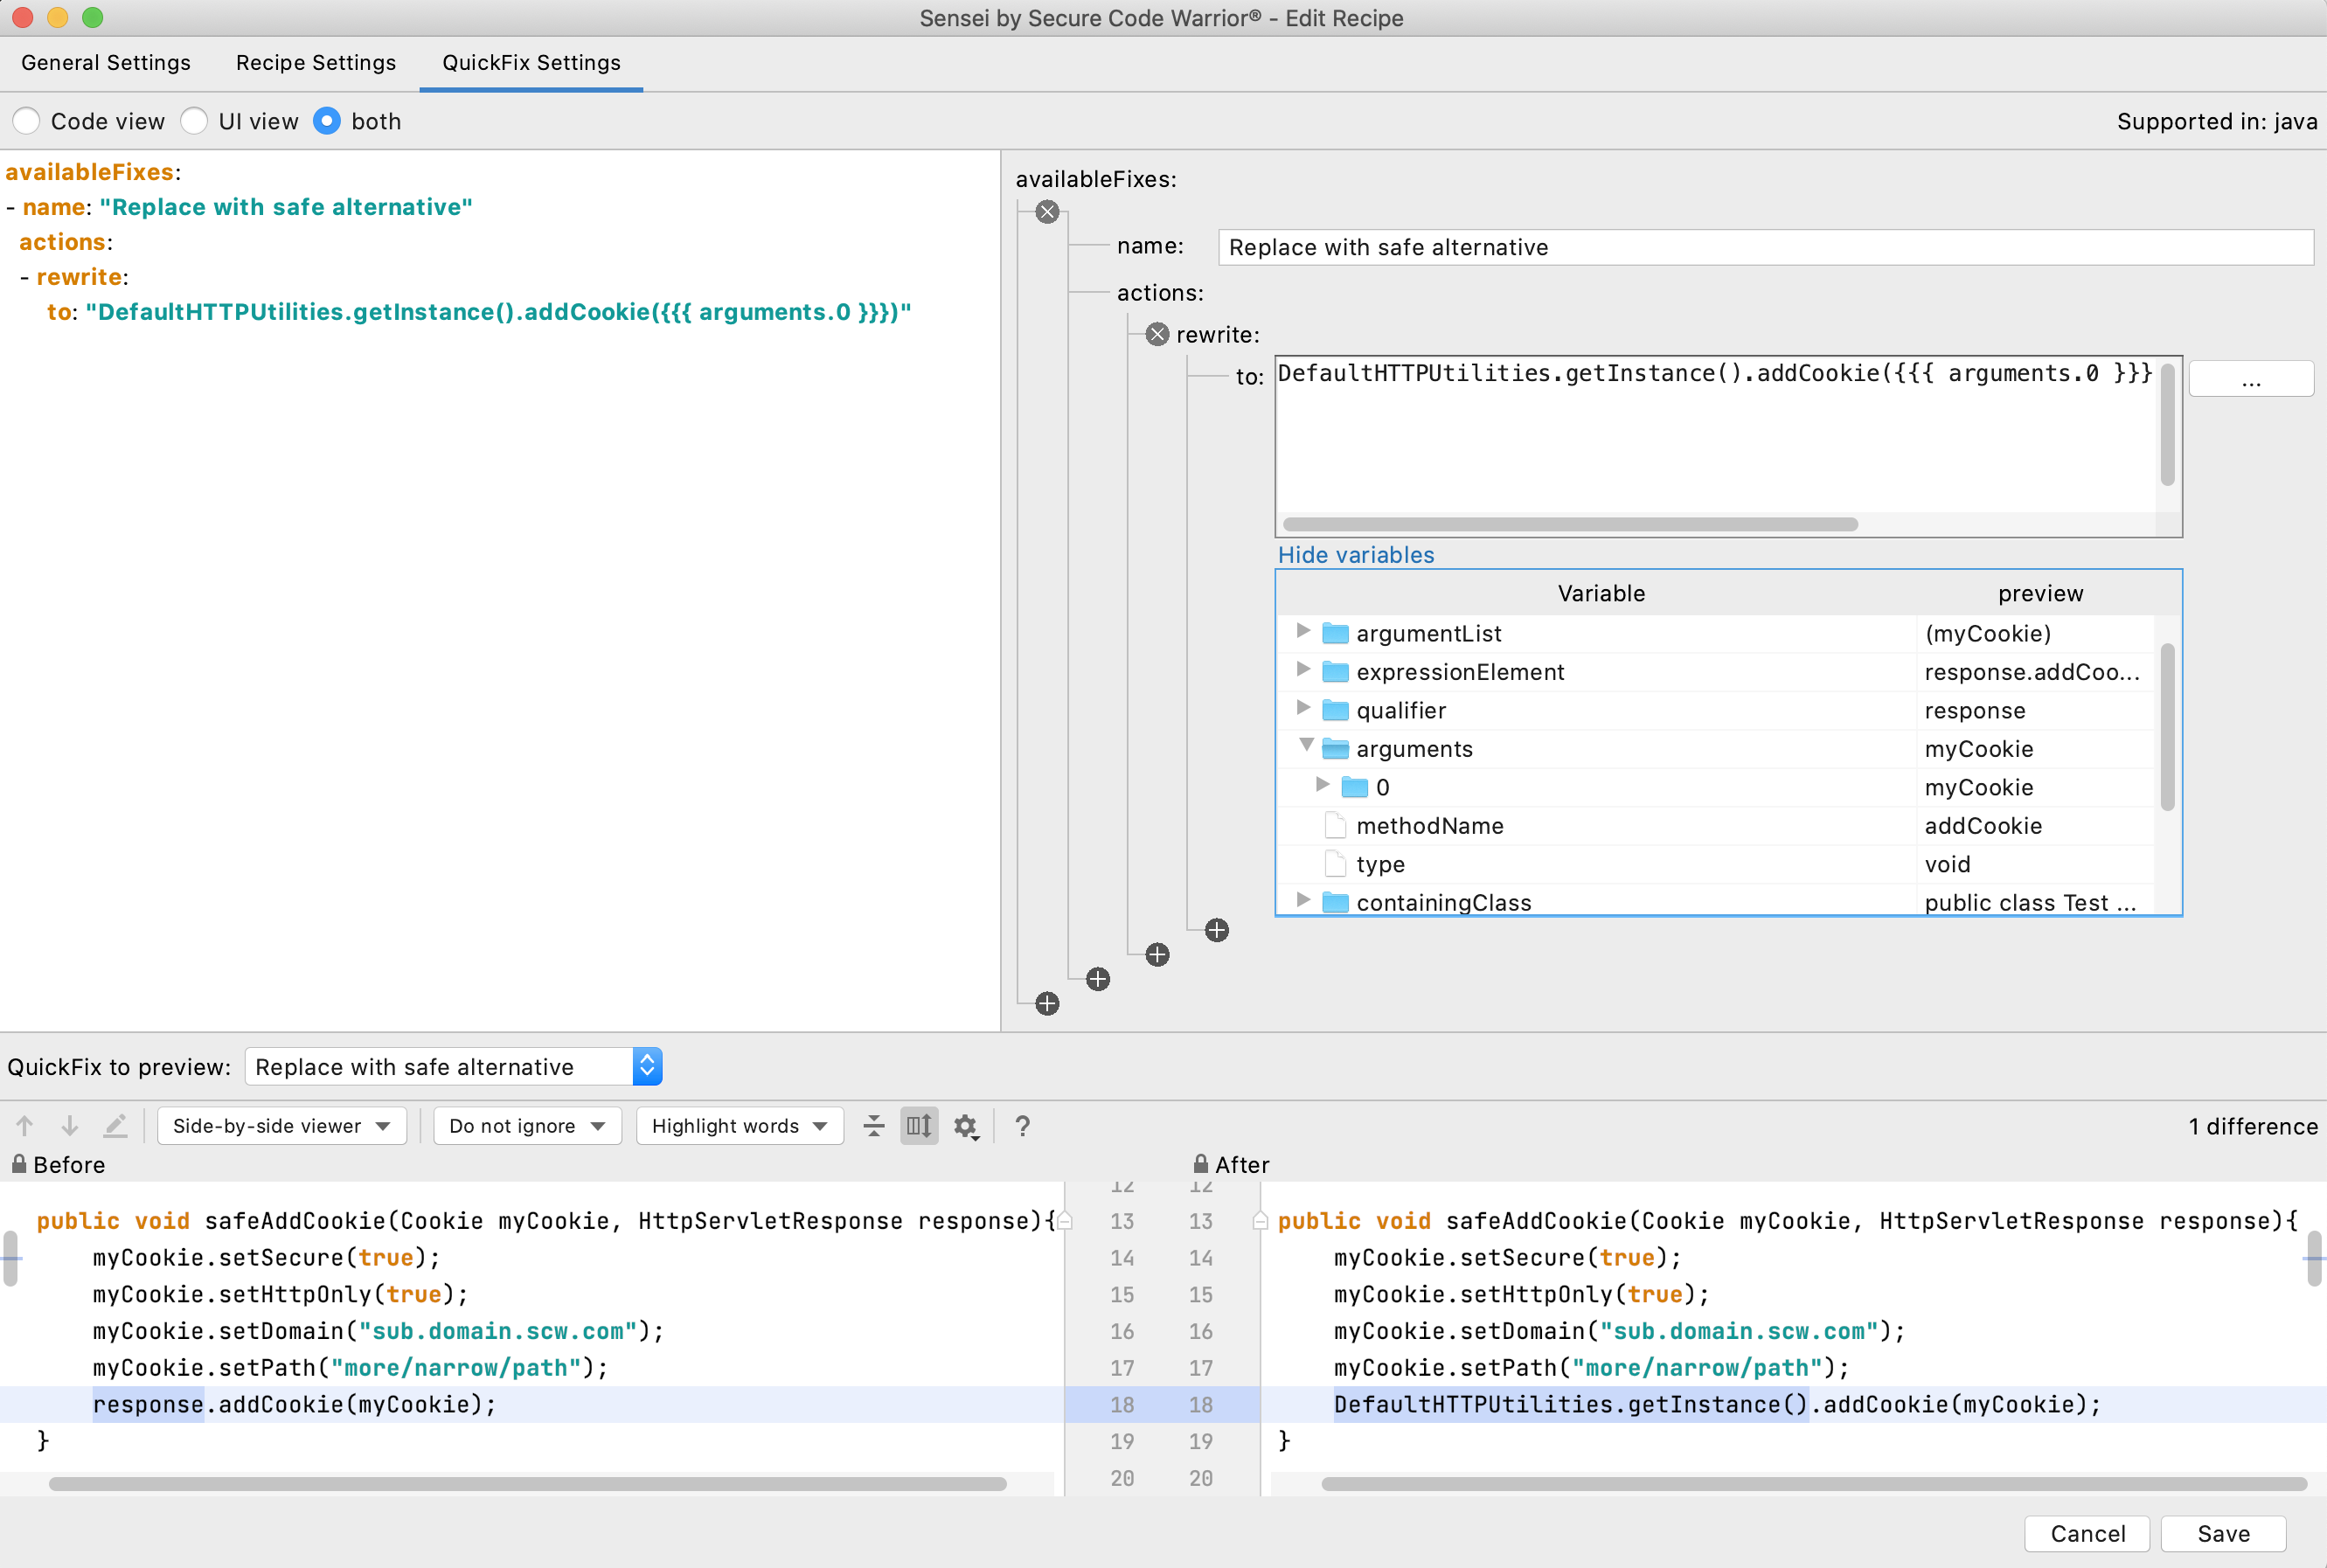
\includegraphics[width=\textwidth]{createfix.png}
  \includegraphics[width=\textwidth,page=5]{04-tools/figures/figures1.pdf}
  \caption[Fix creation window]{The fix creation window allows the recipe writer to reuse parts of the original code.}
  \label{fig:createfix} 
\end{figure}

Finally, besides the trigger and the fix, there are also a number of general settings for the recipe that can be configured, as shown in Figure~\ref{fig:generalsettings}.
Some examples are the name, descriptions, the category of a related vulnerability, overriding recipes, and scopes.
All of these features are related to the usability of the developer and will be discussed in the following sections.

\begin{figure}
  \centering
  %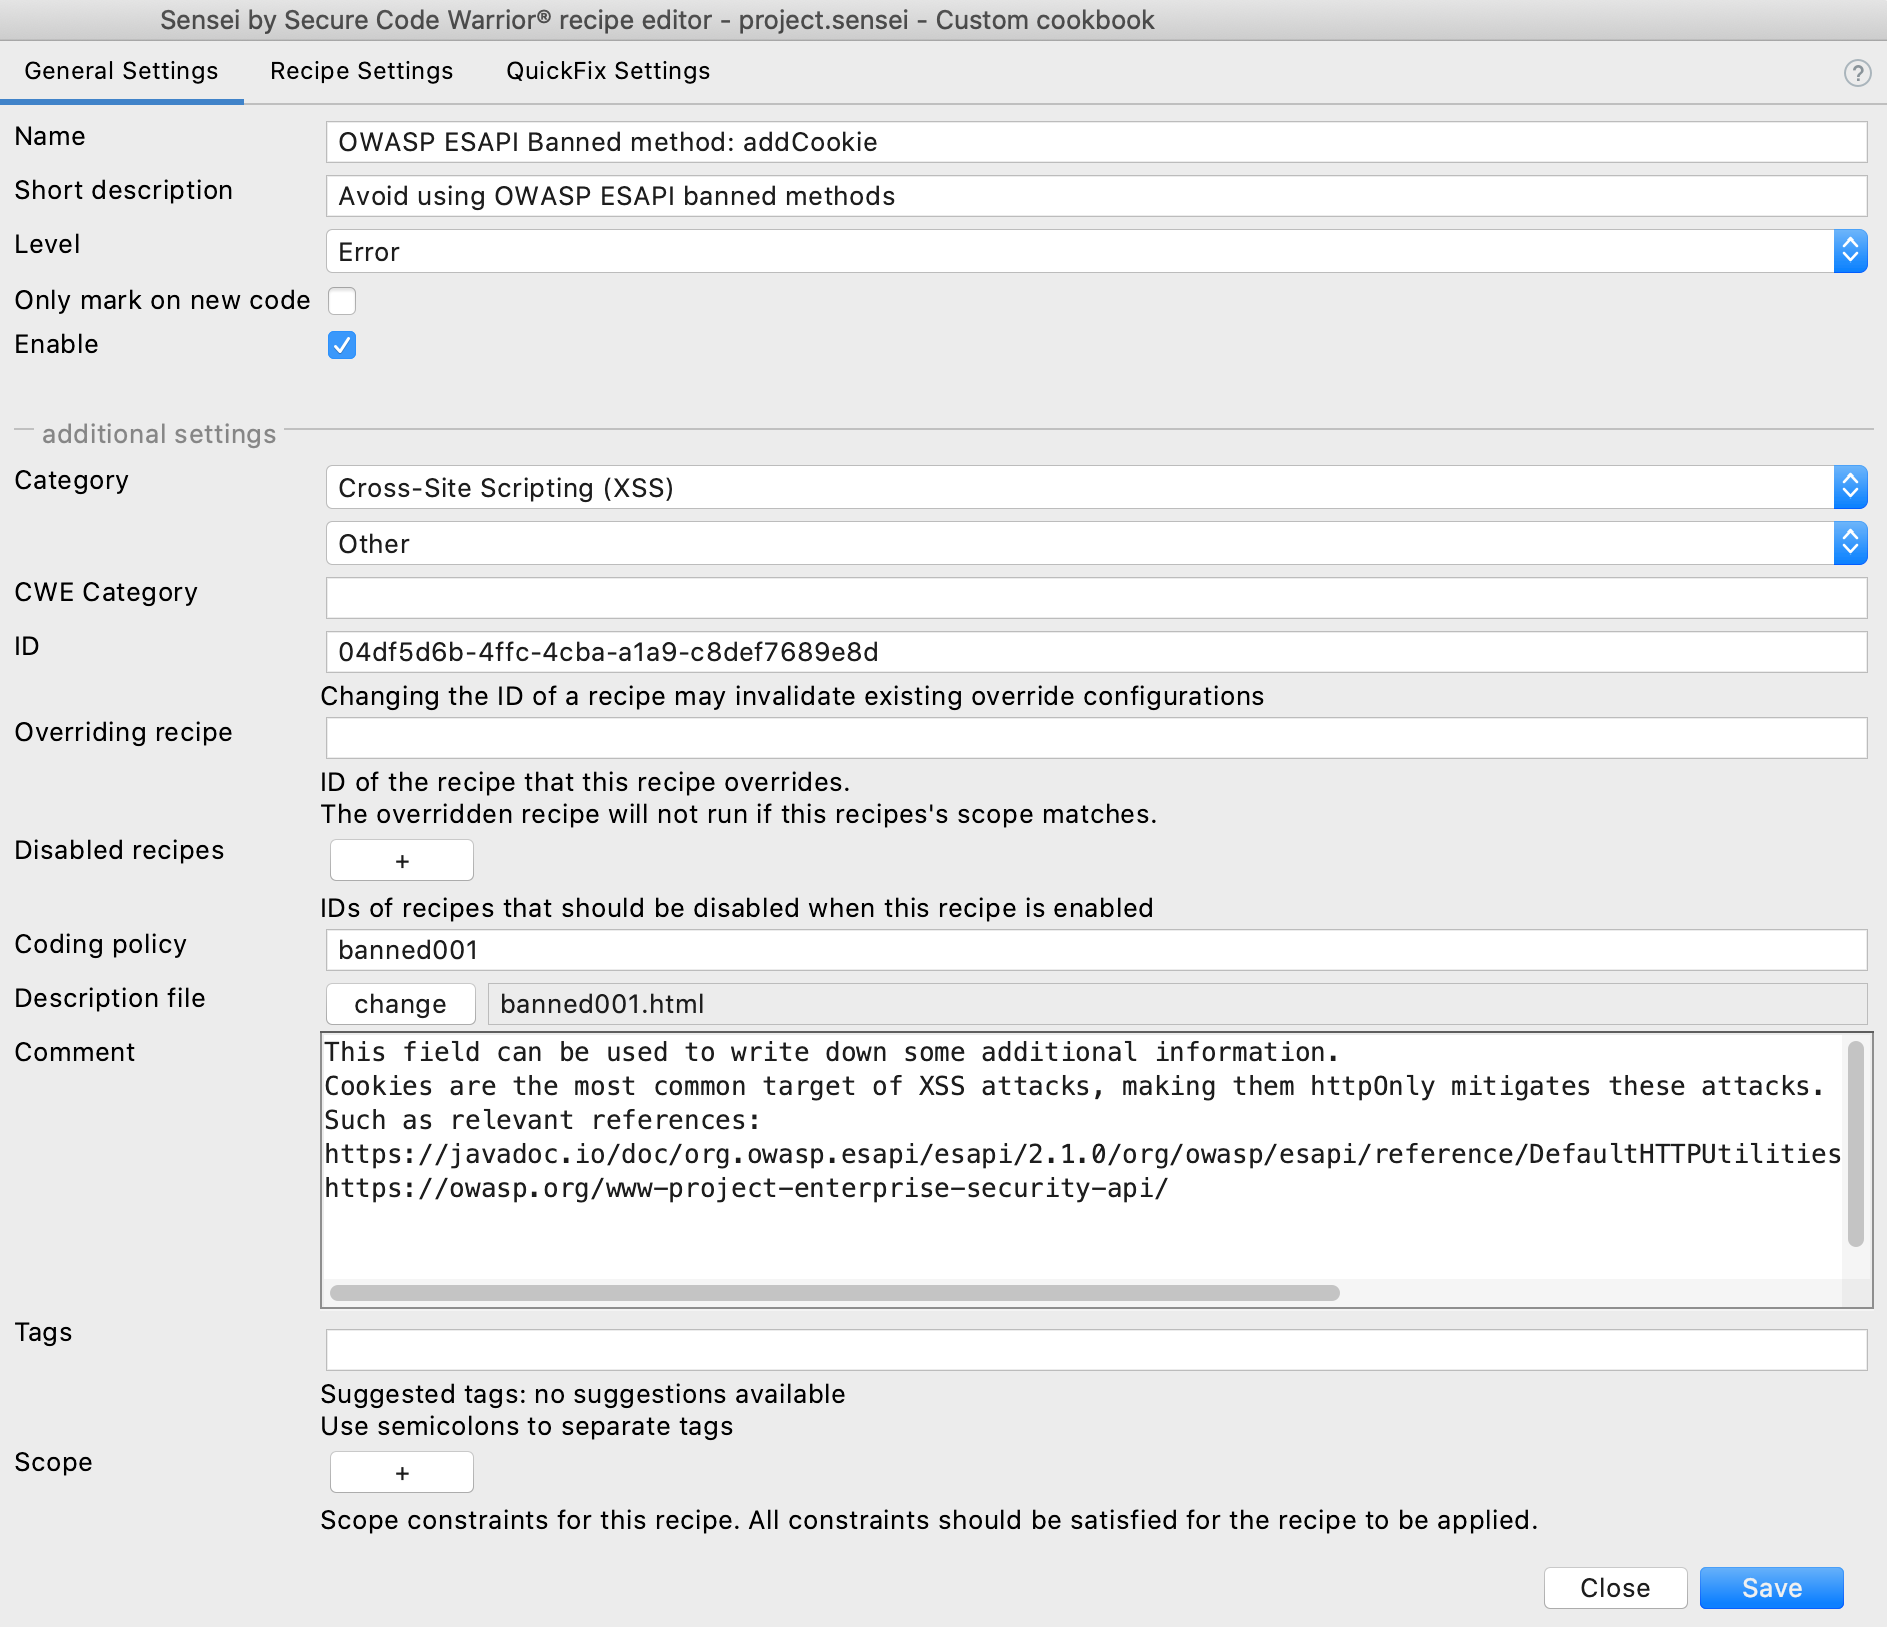
\includegraphics[width=\textwidth]{rulegeneral.png}
  \includegraphics[width=\textwidth,page=8]{04-tools/figures/figures2.pdf}
  \caption[General recipe settings]{Some additional settings are available in the recipe editor mostly related to usability of the developer.}
  \label{fig:generalsettings} 
\end{figure}

We have observed that the context-aware recipe wizard has greatly sped up the recipe creation process.
In practice, creating new recipes often starts from a bad code example, either when fixing a vulnerability or while reviewing the code of a colleague.
The recipe writer can then simply open the recipe creation wizard from this example.
The live previews also greatly improve the usability, since before they were introduced, to create a finished recipe the recipe writer was required to go back and forth several times to test the recipe in the \gls{ide} and adjust it in the recipe editor.

\subsection{Verifying recipes}
To check the recipes, our tool reuses the \gls{ide} syntax checking features.
When a developer writes new code, the \gls{ide} rebuilds the \gls{ast} and computes the changes compared to the previous version.
A limited \gls{ast} of the changes, containing the necessary symbol information, is then passed on, allowing tools to only analyze the changes.
On this \gls{ast}, a combination of specialized light-weight versions of existing analysis techniques is used such as taint analysis, data flow analysis, and control flow analysis to verify the recipes in real time.

\subsection{Managing recipes}
\label{sec:manager}
%\todo[inline]{could you please explain how a developer would know where to consult for recipe sets, depending on which APIs are being used in a program? Bjorn: Mijn originele vraag is nog steeds geldig: Waarom denk je hier niet explicieter op te antwoorden? De vraag is volgens mij hoe developers de sets kunnen consulteren, hoe ze weten welke sets voor hen toepasbaar zijn. De vraag van de reviewer was niet hoe de regels tot stand komen.}
In the paved path methodology, guidelines can be put in place at the start of the project.
If not, at the very least, relevant guidelines should be created each time a new feature is going to be developed.
Together with those guidelines, Sensei recipes should be created as well.
The recipes, however, can also be used by the developers themselves, as a way to share knowledge.
When they develop new \glspl{api}, additionally to documentation, developers can also add Sensei recipes to the project that help their colleagues use these \glspl{api} as intended.

We also recommend to make Sensei recipes part of the remediation process when problems are found by security testing or reported through bug bounty programs.
It should be part of the process to create a recipe that prevents this same vulnerability from occurring in the future.
Currently, it is often the case that security experts run the security scans.
When problems are found, these experts guide the developers by providing them with informal, broadly applicable guidelines and checklists.
These instructions sometimes use security jargon that might not be clear to all developers, and even if they are understood, that does not guarantee the developer will be able to apply them in practice.
In the paved path methodology, security experts and developers should work together to create \gls{api}-level guidelines instead.
As part of this process, to communicate these guidelines to the rest of the team, Sensei recipes can be created as well.

For existing projects, we recommend companies to start with no recipes and use existing data on the security of their project as a starting point.
This could be the report of a penetration test, or results of vulnerability scans.
While resolving these issues in the code, developers and security experts can start building the first recipes.
Some clients are hesitant to start with an empty security tool and, despite our recommendations to customize recipes for each project, still wish to receive a starting recipe pack.
For this reason we have created small open-source sets of unopinionated recipes that can be used in all projects\footnote{\url{https://securecodewarrior.github.io/public-cookbooks/}}.
These recipes aid in correctly using the standard libraries of certain popular frameworks (e.g., Java 
\gls{ee}, Android \gls{sdk}, \gls{aws} \gls{sdk}).
This set can be used as inspiration and to get both security experts and developers accustomed to the tool, but usually it does not flag many issues.

Considering the different sources of recipes, developers can have recipes imposed by management and/or by the security team, as well as recipes distributed among the developers per team or project.
On top, there is the open-source cookbooks that can be used as a starting point during the pilot program.
To make the management of recipes easier, we group recipes into cookbooks.
Instead of distributing recipes one-by-one, this allows for grouping and distributing related recipes more easily. 

In order to manage these cookbooks in the \gls{ide}, a cookbook manager is provided, as shown in Figure~\ref{fig:cookbookmanager}.
Each cookbook is specified by a name and a location.
The developer can enable or disable any cookbook as well as edit recipes in some cookbooks.

\begin{figure}
  \centering
  %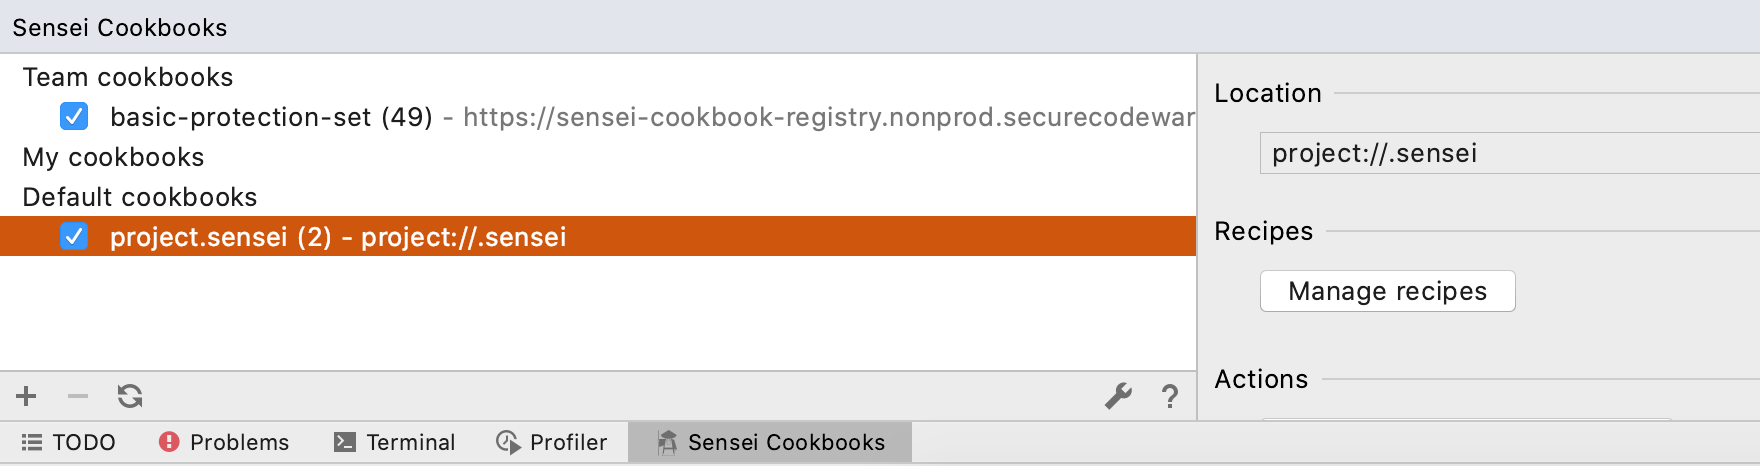
\includegraphics[width=\textwidth]{cookbookmanager.png}
  \includegraphics[width=\textwidth,page=3]{04-tools/figures/figures1.pdf}
  \caption[Cookbook manager]{The cookbook manager in this screenshot contains one remote team cookbook as well as one default cookbook stored in the project structure.}
  \label{fig:cookbookmanager} 
\end{figure}

Cookbooks can be stored locally or remotely.
Remote cookbooks are called team cookbooks and can be loaded from a github project (e.g., \texttt{git@gitserver:cookbooks|master|recipes}) or another remote server location (e.g., \texttt{https://remote.com/recipes.zip}).
Remote cookbooks are only recommended to distribute generally applicable cookbooks, since remote recipes are not editable by the developers and are instead read-only.
Any updates to the remote cookbooks are automatically pushed to all the developers.
Locally stored cookbooks are editable and can be specified by a local path (e.g., \texttt{/Users/dev/recipes}) for personal cookbooks or a path starting from the project root (by default \texttt{project://.sensei}) for default cookbooks for a project.
Local cookbooks are editable which means they can also be enabled on a recipe-by-recipe basis.
It is advised to store project specific recipes as part of the project.
This way, the recipes are always available, up-to-date with the code, and following the same flow as regular code (e.g., branch, review, merge).
When recipes follow the same flow as the code, new \glspl{api} and the recipes needed to use them properly can be added to the project and reviewed as a whole. 

The paved path methodology encourages customization of the recipes at project level.
Previous research and experience have shown that customization at at this level is the most successful.
This provides the needed flexibility to tailor the enforced coding guidelines to the code, but also ensures that the team has a joint approach to how the code for a project should be developed~\cite{sadowski2015tricorder}.
Individually customized recipes might lead to disagreements, while company-wide recipes might be too general to be easily applied.

It is possible for a recipe to be configured to disable other recipes, as shown in the general settings in Figure~\ref{fig:generalsettings}.
This feature can be used to improve remote, read-only recipes.
It is possible that such a recipe is not fully applicable to the project, e.g., because it requires too many manual adaptations.
It is then possible to create a replacement recipe that can be distributed to one team or project and disables the original recipe when it is active.
To facilitate this, an option in the quick-fix menu is added to copy remote recipes to a local cookbook, as shown in Figure~\ref{fig:copyrecipe}.
This option can easily be hidden in the settings.
The clone recipe window, shown in Figure~\ref{fig:clonewindow}, provides an option to automatically disable the original recipe it is copied from.
When a remote recipe is disabled or replaced, the author of this recipe should be notified.
It is possible that it is a generally applicable improvement and the recipe can be updated accordingly for other teams or projects that use it in a remote cookbook.
An additional quick-fix option will be added in the future to disable a recipe.

\begin{figure}
  \centering
  %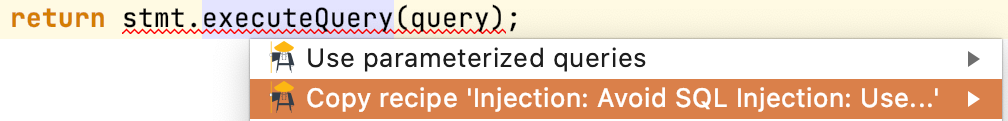
\includegraphics[width=\textwidth]{copyrecipe.png}
  \includegraphics[width=0.9\textwidth,page=4]{04-tools/figures/figures1.pdf}
  \caption[Copy recipe option in the quick-fix menu]{For remote recipes, the quick-fix menu offers a ``Copy recipe" option.}
  \label{fig:copyrecipe} 
\end{figure}

\begin{figure}
  \centering
  %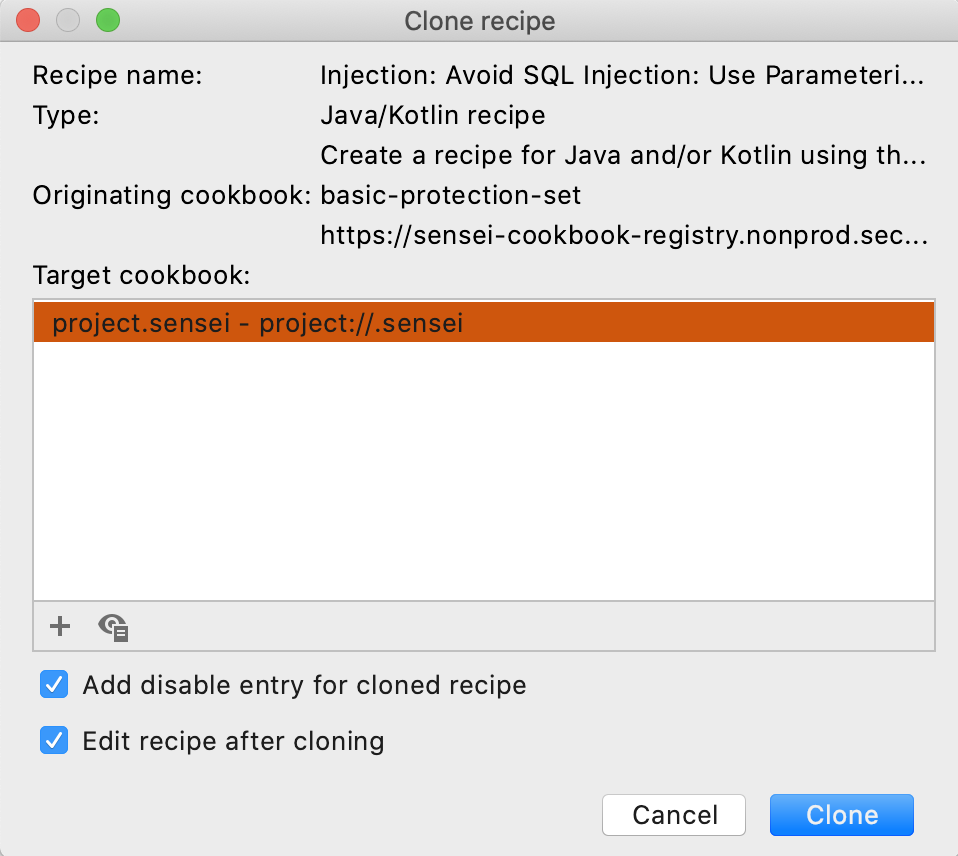
\includegraphics[width=0.75\textwidth]{clonerecipe.png}
  \includegraphics[width=0.75\textwidth,page=2]{04-tools/figures/figures1.pdf}
  \caption[Clone recipe window]{The clone recipe window allows the recipe writer to configure the new recipe to disable the recipe it is copied from.}
  \label{fig:clonewindow} 
\end{figure}

The discussed features to disable recipes have been designed to improve the usability of the tool for developers.
They are in line with the philosophy that developers' productivity benefits from their ability to customize their development environment to their preferences, and to give them a significant amount of freedom in that regard.
In that philosophy, it is preferable to have developers disable some recipes rather then uninstalling or neglecting the tool completely.
Importantly, this does not necessarily result in guideline violations slipping below the radar, since security and management can still have these recipes, as well as complimentary tools, enabled in later phases of the \gls{sdlc}.

\subsection{Explaining recipes}
\label{sec:information}
In order to mark violated guidelines, our plugin makes use of existing \gls{ide} features to flag coding mistakes.
In most \glspl{ide} the code markings by default have three levels of severity: \emph{error}, \emph{warning}, and \emph{information}.
We recommend to mark coding guideline violations as errors.
Traditional error-level markings are usually immediately addressed by the developer, while warning-level markings are more frequently ignored~\cite{whitney2018embedding}.
This is the case because error-level warnings in an \gls{ide} typically indicate a problem in the code that will result in a compilation failure.
Currently error markings by our tool still allow successful compilation of a project, but several clients have requested for the markings to result in compilation failures, equivalent to errors marked by the \gls{ide} itself.
This is not surprising, as it is in line with the default behavior of popular \glspl{ide} such as Visual Studio.
When Visual Studio's C compiler compiles code that uses the insecure \texttt{sprintf} function, it throws a compilation error warning the developer that the function may be unsafe.

An example marking can be seen in Figure~\ref{fig:publicactivity}, where the opening \texttt{<activity>} tag in \gls{xml} code is marked as an error.
This marking makes the code fragment stand out and attracts the developer's attention.
In the example, the Android activity is configured as a public activity by setting the \texttt{exported} attribute to \texttt{true} but not configuring an intent filter.
In \gls{xml} code, like in this example, it is advised to only mark the opening tag, and not the entire \gls{xml} tag and its content.
This would overwhelm the developer, and it would not be clear which part of the code is lacking. 

\begin{figure}
  \centering
  %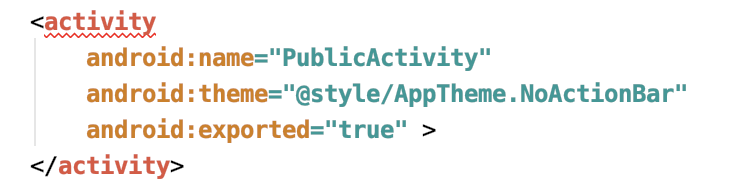
\includegraphics[width=.75\linewidth]{publicactivity.png}
  \includegraphics[width=0.75\textwidth,page=3]{04-tools/figures/figures2.pdf}
  \caption[Error marking on an XML opening tag.]{\Gls{xml} recipes can be configured to mark the opening tag only (shown in the figure), the opening tag and the closing tag, or both tags and their entire content.}
  \label{fig:publicactivity} 
\end{figure}

Permanent markings, that remind developers of security implications of their decisions, should be marked as information.
To continue on the example of private and public activities, in the code file that implements the activity, we mark the class definition at the information level.
Hovering over the marking informs the developer whether the activity is configured as public or private, and provides a direct link to detailed information about the security implications.
This marking is shown in Figure~\ref{fig:infomarking}.
Note how the markings are clearly visible and noticeable, but at the same time non-intrusive to developers already used to their \gls{ide} flagging code fragments.

\begin{figure}
  \centering
  %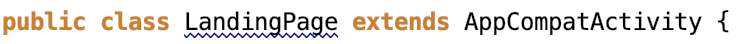
\includegraphics[width=0.80\linewidth]{infomarking2.png}
  \includegraphics[width=0.8\textwidth,page=10]{04-tools/figures/figures1.pdf}
  \caption[Marking at the information error level]{The information error level marking is clearly visible but at the same time non-intrusive, as this is a permanent marking that can not be resolved.}
  \label{fig:infomarking} 
\end{figure}

The marking of code is accompanied by three different descriptions.
This information is important to ensure the continued use of the tool~\cite{whitney2018embedding,layman2007toward}.
Developers build trust with analysis tools, and this trust is quickly lost if they do not understand the tool’s output~\cite{bessey2010few}.
The first description is the short error description, i.e., the text that appears when the developer hovers their mouse pointer over the marked code.
It should be just one line.
The purpose of this description is to attract attention, inform the developer that something should be addressed, not to explain how to address it.

We have learned through user feedback that it is most effective to attract the user's attention by starting with the “why”~\cite{RSAvideo}, the reason the code is marked and should be addressed.
In the past the short description used to indicate the possible vulnerability class, for example “Could lead to SQL injection”. 
We believed that starting with the potential consequences, makes the developers realize the severity of their mistake and encourages them to immediately address it.
However, as explained in Section~\ref{sec:communication}, security jargon should be avoided when communicating to developers.
The feedback in all of the descriptions should be targeted at developers, and hence the focus should be on the guidelines that were put in place, on the paved path.
A better short description is hence, “Violates a guideline on data retrieval”, as depicted in Figure~\ref{fig:shortdescription}.

\begin{figure}
  \centering
  %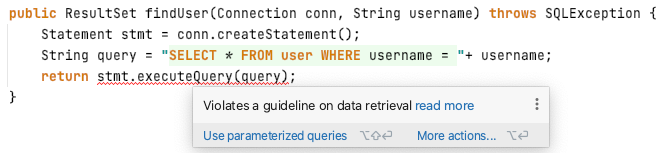
\includegraphics[width=\linewidth]{shortdescription2.png}
  \includegraphics[width=\textwidth,page=14]{04-tools/figures/figures2.pdf}
  \caption[Short description of a recipe]{The short description of a recipe is visible when hovering over a marking. It should attract the developers attention but avoid security jargon. Instead, the developer can be reminded of guidelines that are in place.}
  \label{fig:shortdescription} 
\end{figure}

Next to the short description a “read more” link is created by the \gls{ide} for the interested developer.
Upon clicking this link, a pop-up is opened to show a more elaborate \gls{html} page.
This is the second description.
Figure~\ref{fig:fulldescription} shows an example.
This description is called the full coding guideline.
The page starts with a short abstract, stating in one sentence what should be done, such as “Secure coding practices prescribe that queries need to be parameterized”.
The page's next section presents in detail what it means to use parameterized queries and gives an overview of the approved \gls{api} methods.
Small code examples are included as well, since previous research has shown examples are the fastest way for developers to understand a problem~\cite{whitney2018embedding}.
The goal of this description is after all to help developers find out quickly how to comply to the coding guideline without spending much time or effort.
This is crucial for a security tool to feel well integrated into developer workflows.
The last section of the description contains a list of possible consequences when the developer fails to address this issue.
There is no mention of vulnerabilities or exploits until this point.
Each item in the list contains a link to the \gls{scw} training platform to learn more about the vulnerabilities and how they are exploited.
This way an interested developer (with too much time on their hands?) can still easily find the necessary information to learn the details of each vulnerability and the possible attacks.
Following this training would require a context switch and would likely hurt developer productivity.
In the future the integration between the \gls{scw} training platform and the Sensei \gls{ide} plugin can be improved as described in the perspectives in Section~\ref{sec:its-integration}.

\begin{figure}
  \centering
  %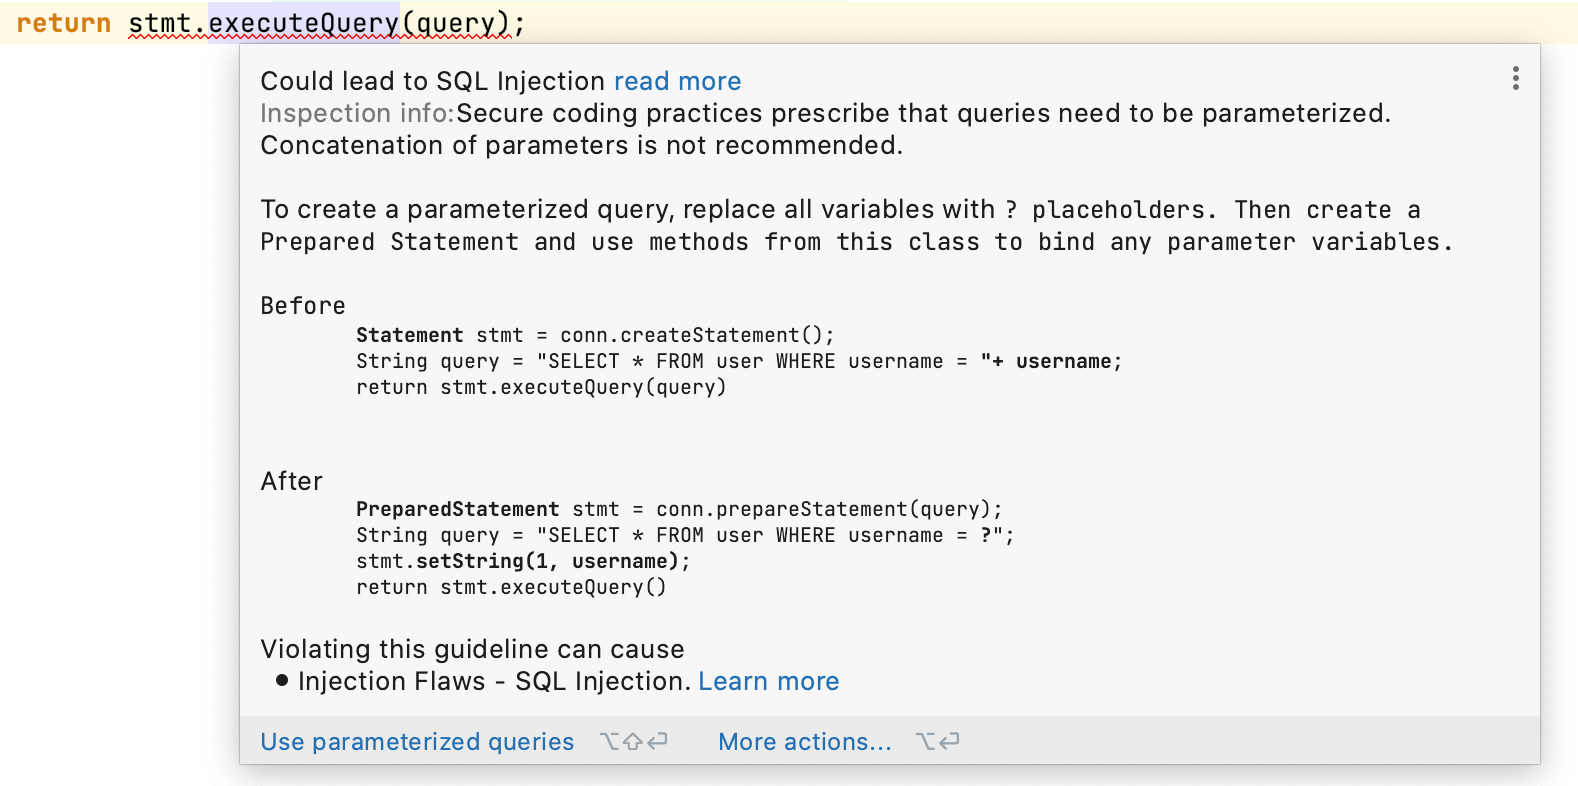
\includegraphics[width=\textwidth]{guideline.png}
  \includegraphics[width=\textwidth,page=7]{04-tools/figures/figures1.pdf}
  \caption[Example of the full coding guideline.]{The full coding guideline is a more elaborate \gls{html} page that explains the guideline in more detail and provides code examples.}
  \label{fig:fulldescription}
\end{figure}

The third description is visible to the developer when they press the \gls{ide}’s key combination (Windows/Linux: Alt+Enter, Mac: Option+Enter) to start resolving the issue.
A drop down menu appears, containing the possible quick-fixes' descriptions.
%A "copy recipe" option is available as well, and for local recipes there is also additionally an "edit recipe" option, both of these can be disabled in the Sensei settings.
IntelliJ also provides options to disable inspections locally or globally. Figure~\ref{fig:qfdescription} shows an example.
In this menu we provide a very short description of the actions that will be performed when this code transformation is chosen, such as “Use parameterized queries”.
A brief yet descriptive quick-fix description allows developers to decide quickly whether the fix is appropriate for them.
If the effects of applying the quick-fix are well understood, the developer will trust the tool and apply the fixes more often.
Sometimes the developer needs to choose between different possible solutions.
However, it is advised to keep the number of fixes as low as possible, as to not complicate the issue unnecessarily.

\begin{figure}[t]
  \centering
  %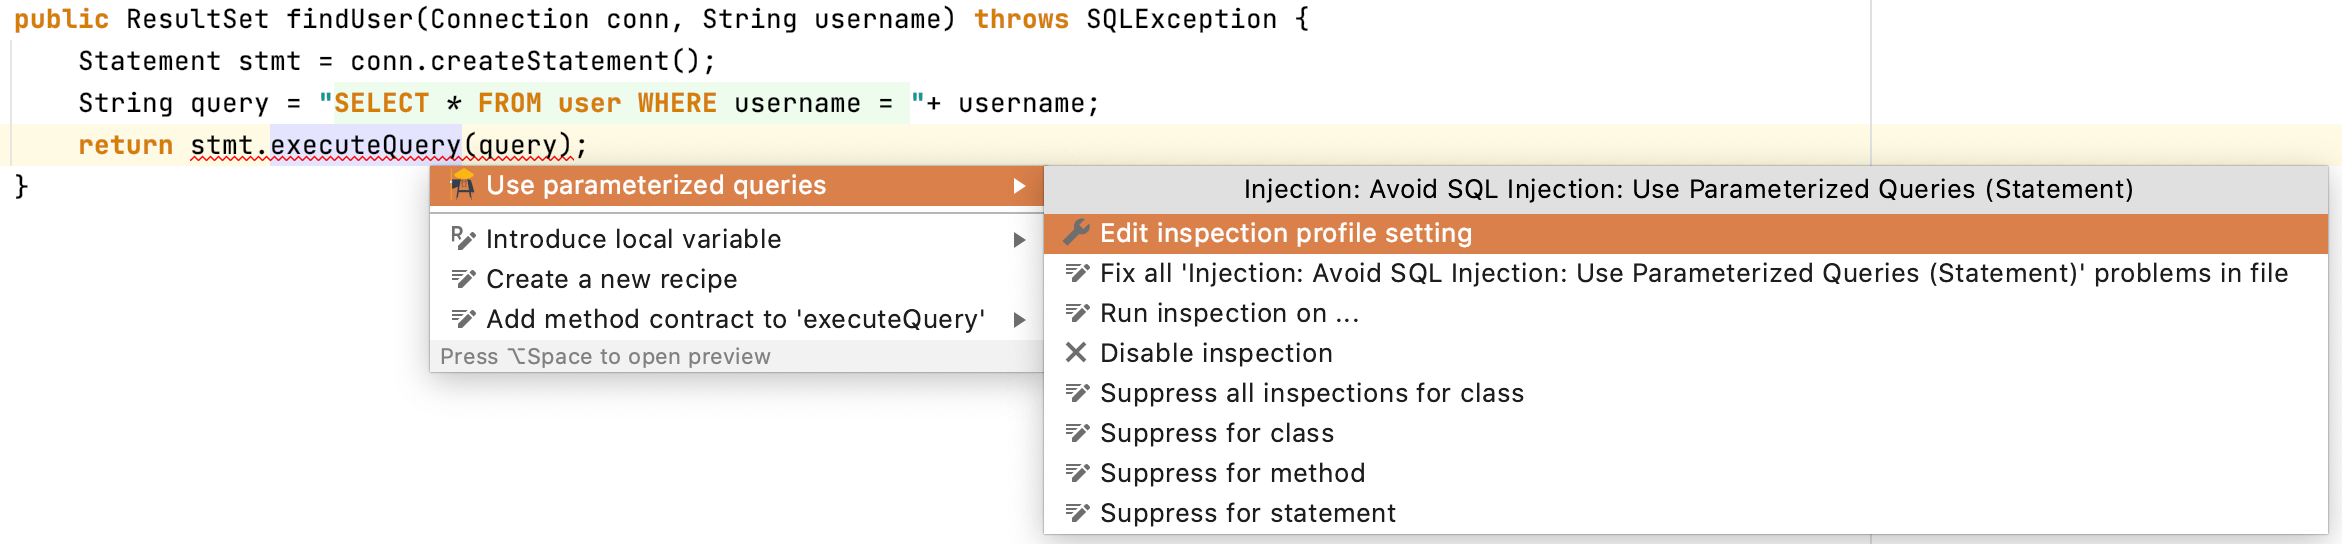
\includegraphics[width=\textwidth]{quickfixmenu.png}
  \includegraphics[width=\textwidth,page=5]{04-tools/figures/figures2.pdf}
  \caption[Example of the quick-fix description.]{The quick-fix description briefly describes the actions that will be performed when each option is chosen. IntelliJ also offers a feature to suppress markings of any inspection (Sensei or otherwise).}
  \label{fig:qfdescription} 
\end{figure}
